\documentclass[11pt,letterpaper]{article}
\PassOptionsToPackage{hyphens}{url}
\usepackage[margin=.83in,top=.8in,bottom=.8in,headheight=15pt]{geometry}
\usepackage[T1]{fontenc}
\usepackage{lmodern,amsmath,amssymb,mathtools,bm,booktabs,array,graphicx,tikz}
\usetikzlibrary{arrows.meta,positioning,calc,decorations.pathreplacing,patterns}
\definecolor{ink}{HTML}{17344D}\definecolor{accent}{HTML}{087E8B}\definecolor{pale}{HTML}{EDF5F5}\definecolor{gold}{HTML}{AD6B19}
\providecommand{\dd}{\,\mathrm{d}}\providecommand{\R}{\mathbb{R}}
\providecommand{\E}{\mathbb{E}}\providecommand{\Var}{\operatorname{Var}}
\providecommand{\Cov}{\operatorname{Cov}}\providecommand{\diag}{\operatorname{diag}}
\providecommand{\norm}[1]{\left\lVert#1\right\rVert}
\providecommand{\abs}[1]{\left|#1\right|}
\usepackage{microtype,hyperref,fancyhdr,enumitem,amsthm,sectsty,needspace}
\allsectionsfont{\raggedright}
\hypersetup{colorlinks=true,linkcolor=ink,urlcolor=accent,pdfauthor={Zan Ahmad},pdftitle={Local convolutional segmentation and geometric error / Lecture notes}}
\setlength{\parindent}{0pt}\setlength{\parskip}{6pt}\linespread{1.07}
\setlist{itemsep=3pt,topsep=4pt,leftmargin=*}
\emergencystretch=2em\clubpenalty=10000\widowpenalty=10000
\pagestyle{fancy}\fancyhf{}\fancyhead[L]{\small Computational Cardiology}\fancyhead[R]{\small Lecture 12}
\fancyfoot[L]{\footnotesize Zan Ahmad}\fancyfoot[R]{\footnotesize\thepage}\renewcommand{\headrulewidth}{.3pt}
\newtheorem{proposition}{Proposition}\newtheorem{theorem}{Theorem}\newtheorem{lemma}{Lemma}
\theoremstyle{definition}\newtheorem{definition}{Definition}\newtheorem{example}{Example}
\numberwithin{equation}{section}
\begin{document}
{\small\scshape Computational Cardiology\hfill Lecture 12}\par\medskip
{\raggedright\hyphenpenalty=10000\exhyphenpenalty=10000\LARGE\bfseries\color{ink} Local convolutional segmentation and geometric error\par}\medskip
{\small Lecture notes}\par\bigskip
A shared local classifier turns image patches into a segmentation mask. Its parameters, loss and gradient can be written completely, making the relation between a convolutional rule and geometric error explicit. Overlap, boundary distance and connectivity then measure different consequences of the resulting mask.

\section{Pixelwise prediction and comparison units}
\hypertarget{note-pixelwise-prediction-and-comparison-units}{}\label{note:pixelwise-prediction-and-comparison-units}
{\small \href{slides.html\#frame=the-output-of-segmentation\&step=1}{Slides for this section}}\par
A segmentation assigns a class to every pixel. Its output is a spatial mask, whereas image classification supplies one label for a whole image. That distinction changes evaluation: a method can classify the presence of a shape correctly while placing its boundary poorly. We use original synthetic ellipses to isolate the mechanics. Each reference mask is known from the generator; blurred intensities and random noise make the segmentation nontrivial. The reference is exact for this generator, not a substitute for clinical annotation or a model of all cardiac structures.

Our baseline labels intensities at least 0.5 as foreground. It has no fitted parameters and is deliberately easy to inspect. The second method learns a shared local rule from labeled training images. Both methods receive the same held-out images and use the same physical grid, so a comparison is interpretable. We inspect the first test image by a predeclared index rather than choose the most flattering output after computing scores. The full result file retains per-image metrics to make disagreement visible.

For an image with $M$ pixels, a segmentation predicts a vector in $\{0,1\}^M$, while image classification predicts one label. A local segmentation rule can improve average pixel agreement without preserving every geometric feature needed by a later physical model.
\section{A shared local linear predictor}
\hypertarget{note-a-shared-local-linear-predictor}{}\label{note:a-shared-local-linear-predictor}
{\small \href{slides.html\#frame=a-local-shared-predictor\&step=1}{Slides for this section}}\par
At each pixel, collect a three-by-three neighborhood, subtract the fixed intensity center 0.5, and flatten the nine values into a vector. A dot product with nine shared weights plus one shared bias produces a logit. A sigmoid maps that logit into a number between zero and one, and a predeclared probability threshold of 0.5 produces a mask. The weights are reused at every location; there are ten fitted parameters, not ten new parameters per pixel. The PyTorch Conv2d reference calls this unflipped sliding operation cross-correlation. Our implementation follows that convention in NumPy.

Reflect padding supplies a one-pixel border, allowing the output to retain the 24-by-24 input shape. Padding is an assumption about missing context and should be recorded. The local rule cannot recognize a distant anatomical relationship outside its three-by-three receptive field. Its sigmoid output is a model score; this lesson does not establish probability calibration. Larger convolutional networks combine features across multiple scales. U-Net's original architecture combines a contracting path with an expanding path and corresponding fine-scale features. That reading provides context, while our executable scaffold remains a single learned layer.

\[
z_i=\mathbf{w}^{T}\mathbf{x}_i+b,\qquad p_i=\frac{1}{1+e^{-z_i}}
\]
Each patch has nine dimensionless centered intensities; w has nine weights and b is a scalar. Every pixel uses the same parameters.

If $x_i\in\mathbb R^9$ is the centered patch, the design matrix $X$ has one patch per row. The shared predictor is $z=Xw+b\boldsymbol1$. Weight sharing reduces the parameter count to ten regardless of image size. A translated interior patch receives the same logit; finite-image padding defines how this rule is extended at the border.

\paragraph{Calculation.} A centered patch has nine values equal to 0.2. All nine weights are 0.5 and bias is \ensuremath{-}0.3. Find the output.

The dot product is 9\ensuremath{\times}0.5\ensuremath{\times}0.2 = 0.9.

Adding the bias gives logit 0.6.

The sigmoid gives about 0.6457; thresholding at 0.5 selects foreground.

One shared local rule gives a foreground prediction; it has not identified a particular anatomical object.
\section{Cross-entropy and its derivatives}
\hypertarget{note-cross-entropy-and-its-derivatives}{}\label{note:cross-entropy-and-its-derivatives}
{\small \href{slides.html\#frame=binary-cross-entropy-from-logits\&step=1}{Slides for this section}}\par
For a binary target, cross-entropy penalizes a confident incorrect prediction. We evaluate it directly from the logit with a stable log-add-exp expression, avoiding logarithms of numerically rounded zero probabilities. The training objective averages over all training pixels and adds a small squared-weight penalty. The bias is not penalized. Differentiating the data loss with respect to the logit gives predicted score minus target. Multiplying that residual by the corresponding patch and averaging produces the weight gradient; the bias gradient is the average residual.

The companion initializes parameters at zero, performs 250 full-batch gradient steps at learning rate one, and evaluates validation loss every ten steps. It retains the parameters with the lowest unpenalized validation cross-entropy among those checkpoints. These are explicit teaching choices, not broadly recommended training hyperparameters. A central finite-difference calculation supplies an independent gradient comparison. The check compares all ten derivatives at nonzero parameters; its maximum absolute discrepancy is below one hundred-millionth.

\[
J=\frac{1}{M}\sum_i\left[\log(1+e^{z_i})-y_i z_i\right]+\frac{\lambda}{2}\|\mathbf{w}\|^2
\]
M counts training pixels; y is zero or one; lambda is 0.001. The implementation uses logaddexp for numerical stability.

\[
\nabla_w J=\frac1M\sum_i(p_i-y_i)\mathbf{x}_i+\lambda\mathbf{w},\qquad \partial_bJ=\frac1M\sum_i(p_i-y_i)
\]
Update each parameter by subtracting learning rate times its gradient. Targets affect fitting, not the padding transform.

Writing $p=\sigma(z)$ gives
\[
 \frac{\partial}{\partial z}\{\log(1+e^z)-yz\}=p-y,
 \qquad\frac{\partial^2}{\partial z^2}\{\log(1+e^z)-yz\}=p(1-p)\ge0.
\]
For the augmented matrix $\widetilde X=[X\ \boldsymbol1]$, the data Hessian is $\widetilde X^{\mathsf T}\operatorname{diag}(p_i(1-p_i))\widetilde X/M$. It is positive semidefinite. The squared-weight penalty adds curvature to the weight block but not to the bias. Thus this single-layer fitting problem is convex, although deeper networks generally are not.
\section{Image-level splitting and model selection}
\hypertarget{note-image-level-splitting-and-model-selection}{}\label{note:image-level-splitting-and-model-selection}
{\small \href{slides.html\#frame=the-unit-of-separation-panel-1\&step=1}{Slides for this section}}\par
The generator creates 24 training images, eight validation images and twelve test images with separate seeds. Complete images stay within a single split. Randomly splitting neighboring pixels would let highly related patches from the same image appear in training and testing, answering an easier question. In actual studies, repeated acquisitions from one patient may require grouping at patient level. Here the unit of separation is the independently generated image, and there is no patient population represented.

The test set does not select the iteration, loss penalty or score threshold. After checkpoint selection, both methods are evaluated once under the stated protocol. The fixed baseline has mean per-image Dice about 0.908, while the learned local model reaches about 0.979 on these twelve generated images. This result supports a narrow statement about this generator and noise pattern. It does not prove superiority under another acquisition process, irregular anatomy, an unseen artifact or a rare pathological structure. Report the experiment definition with the numbers.

The learned layer mostly combines nearby evidence, which suppresses isolated noise in these simple examples. Better average overlap can coexist with a systematic size bias: the learned model's mean signed area error is about \ensuremath{-}3.14 percent. A signed mean can also hide cancellation between positive and negative case errors. Inspect individual errors and absolute magnitudes before deciding whether the geometric consequences are acceptable.

Neighboring patches share pixels and a latent image geometry. A random pixel split therefore does not generate independent new-image examples. Splitting entire images makes the held-out unit match the intended generalization unit in this synthetic experiment. Validation selects a checkpoint; the final test images do not participate in that selection.
\begin{center}\begin{minipage}{.98\linewidth}\centering
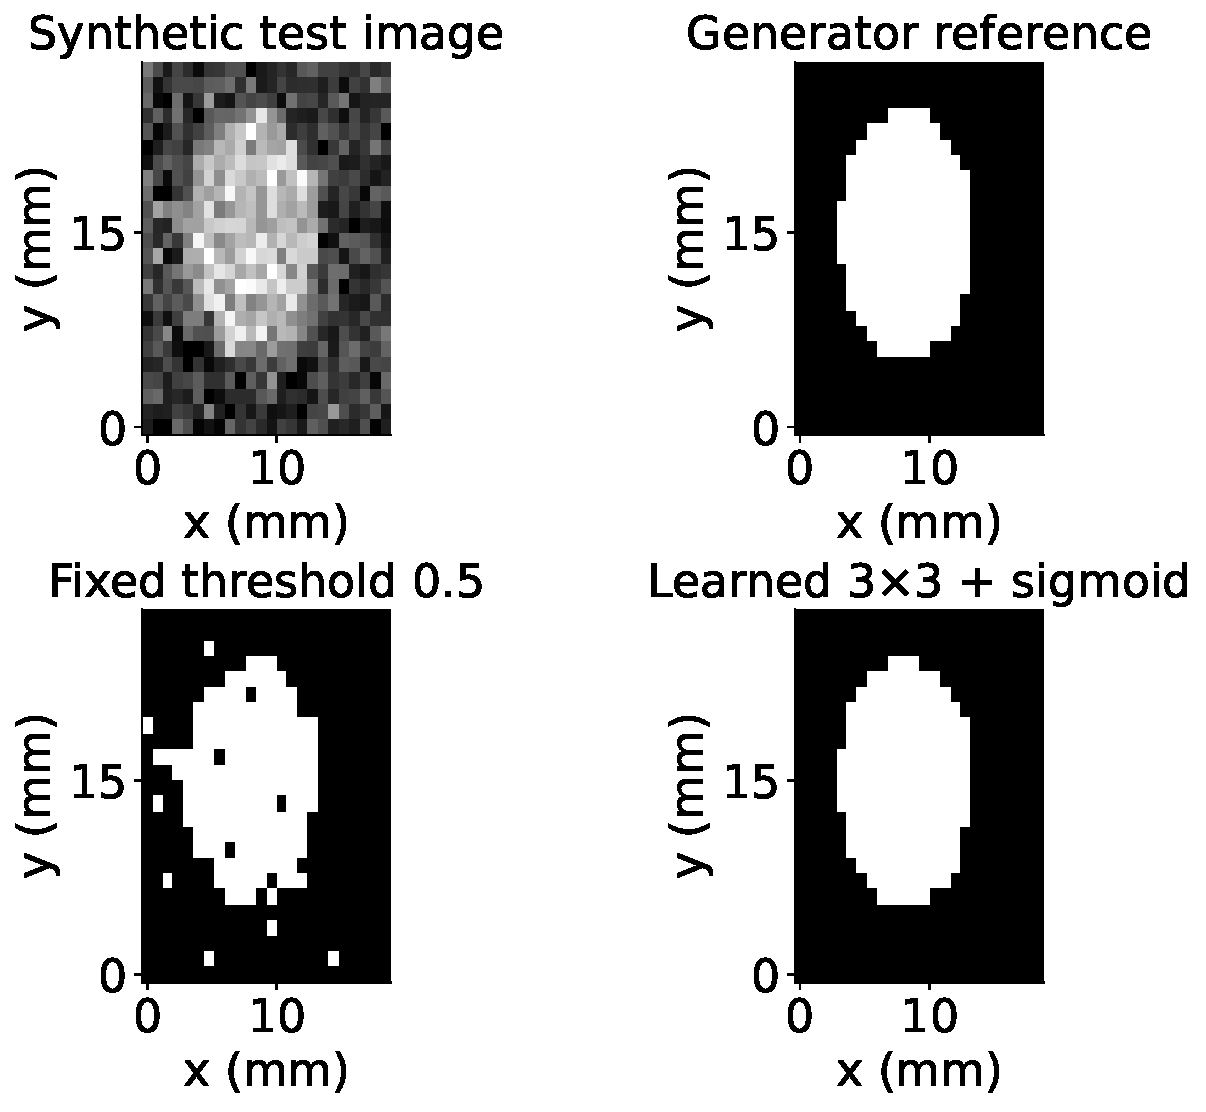
\includegraphics[width=.96\linewidth,height=.57\textheight,keepaspectratio]{segmentation-comparison.pdf}\par\smallskip
{\small Predeclared test image 0, its generator reference, the fixed 0.5 intensity baseline and the learned 3$\times$3-plus-sigmoid prediction. Both use 0.8 mm column spacing and 1.2 mm row spacing; full test summaries are in results.json.}
\end{minipage}\end{center}
\section{Overlap, boundary distance and topology}
\hypertarget{note-overlap-boundary-distance-and-topology}{}\label{note:overlap-boundary-distance-and-topology}
{\small \href{slides.html\#frame=overlap-as-a-set-quantity\&step=1}{Slides for this section}}\par
Dice compares shared foreground with total foreground. It does not use physical distance or encode which part of the object was missed. Our boundary implementation marks foreground pixels adjacent to background under four-neighbor connectivity. We compute nearest-boundary distances in millimeters in both directions, average each direction separately and then average those two means. The Hausdorff distance is the largest nearest-boundary distance in either direction. Both depend on the chosen discrete boundary convention and spacing, so state those conventions with the result.

The companion defines Dice as one for two empty masks and zero if only one is empty. Boundary distance is zero when both are empty and unavailable when only one is empty. Returning an unavailable value prevents a missing object from appearing as perfect boundary agreement. A batch report must count such failures rather than silently exclude them. For nonempty masks, connectivity supplies another essential view. The bridge example removes only four pixels from an 824-pixel reference. Dice remains about 0.9976 and area changes by less than one percent, yet one connected component becomes two.

A disconnected geometry can change which regions communicate in a later transport model. We do not calculate that flow here or infer a clinical effect. The counterexample establishes that overlap alone cannot guarantee preservation of a connection. Even a small mean boundary distance can conceal this specific defect. Decide which geometric features matter for a downstream question before choosing a metric threshold.

\[
\mathrm{Dice}(P,R)=\frac{2|P\cap R|}{|P|+|R|}
\]
P is prediction and R is reference. The both-empty case is explicitly defined as one in this lesson.

For finite boundary point sets $\partial P$ and $\partial R$, define
\[
 d_{sym}=\frac12\left[\frac1{|\partial P|}\sum_{p\in\partial P}d(p,\partial R)+
 \frac1{|\partial R|}\sum_{r\in\partial R}d(r,\partial P)\right].
\]
Hausdorff distance replaces the two means by the maximum of all nearest-boundary distances. Neither formula identifies whether a particular bridge remains connected. Removing four bridge pixels from an $824$-pixel reference gives Dice $1640/1644\approx0.99757$ while changing one component into two.
\begin{center}\begin{minipage}{.98\linewidth}\centering
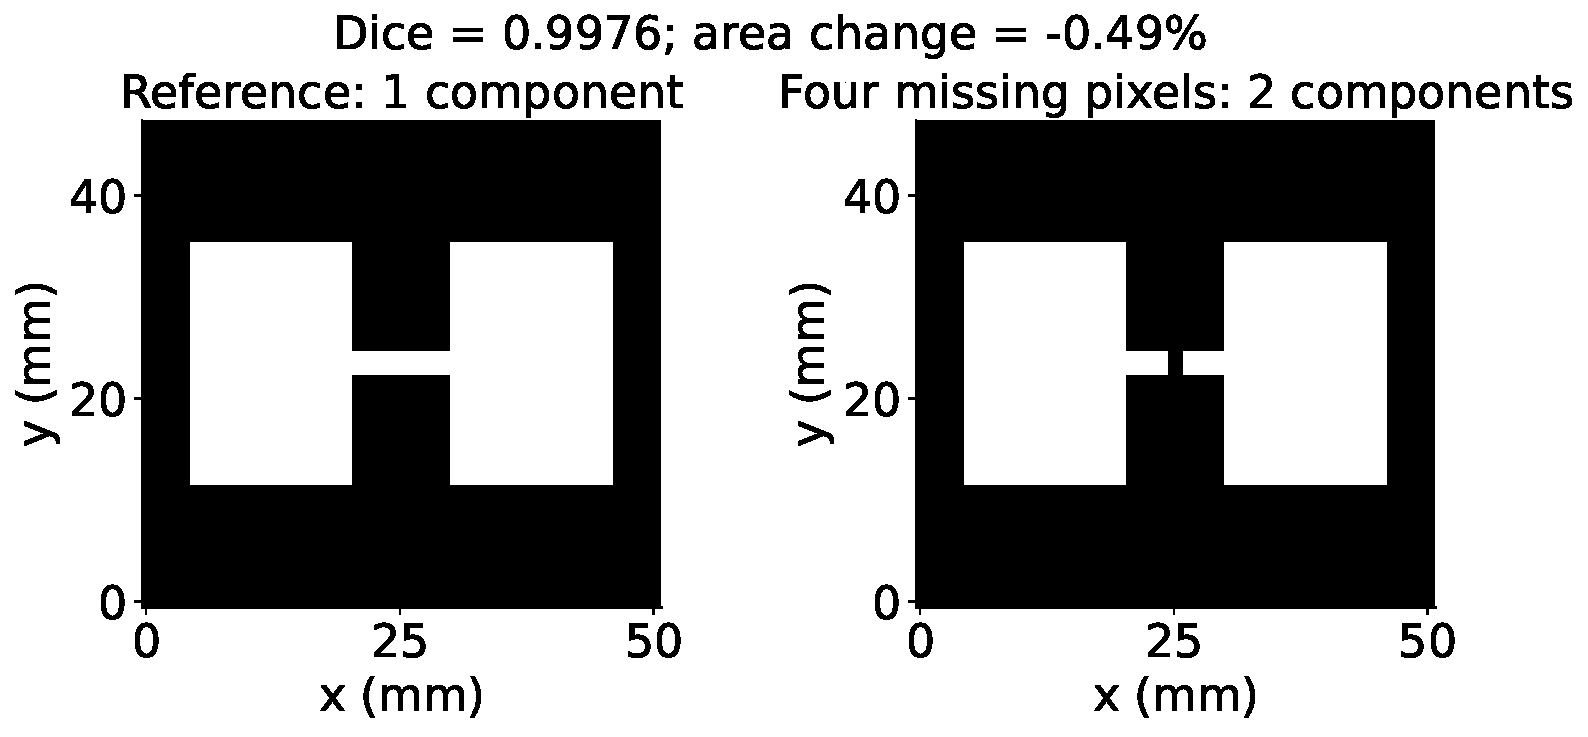
\includegraphics[width=.96\linewidth,height=.57\textheight,keepaspectratio]{connectivity-failure.pdf}\par\smallskip
{\small Removing four pixels gives Dice 0.9976 and signed area change -0.485\%, but changes four-neighbor foreground component count from one to two. This is an original topology counterexample, not a simulated cardiac-flow result.}
\end{minipage}\end{center}
\section{The geometric consequence of a segmentation error}
\hypertarget{note-the-geometric-consequence-of-a-segmentation-error}{}\label{note:the-geometric-consequence-of-a-segmentation-error}
{\small \href{slides.html\#frame=area-bias-and-overlap-are-distinct\&step=1}{Slides for this section}}\par


A physical transport domain requires the connections relevant to its boundary-value problem. Two masks can have nearly equal area and Dice while supporting different paths through the domain. The segmentation comparison therefore concerns both statistical prediction and the geometry inherited by the downstream model. Better mean overlap on this generator does not establish performance on another acquisition process or on rare anatomical features.
\bigskip
\section*{Exercises}
\par\noindent\begin{minipage}{\linewidth}
\subsection*{AC12-E1. Trace one gradient update}
Consider a single patch with all nine centered values equal to 0.2, target y=\allowbreak{}1, zero weights and zero bias. Use learning rate 0.5 and lambda 0.001.

\textbf{a} Find the initial logit, score and data loss.

\end{minipage}\par\medskip
\textbf{b} Compute each weight gradient and the bias gradient.

\textbf{c} Apply the update and find the new logit. Does its direction make sense?

\par\noindent\begin{minipage}{\linewidth}
\subsection*{AC12-E2. Overlap is not a boundary metric}
A reference has 100 foreground pixels. Prediction P has 110, of which 90 overlap the reference. Prediction Q has 100, of which 90 overlap. Both use the same grid.

\textbf{a} Calculate Dice and signed area error for P.

\end{minipage}\par\medskip
\textbf{b} Calculate the same quantities for Q. Does zero area error imply a correct boundary?

\textbf{c} Can the supplied counts determine Hausdorff distance or connectivity? Name the missing information.

\par\noindent\begin{minipage}{\linewidth}
\subsection*{AC12-E3. Audit the split and the metric conventions}
A researcher has three scans from each of ten individuals and randomly assigns pixels to training or testing. They also report a boundary distance of zero when their model predicts no foreground.

\textbf{a} Explain the leakage risk and give an appropriate split unit for testing transfer to new individuals.

\end{minipage}\par\medskip
\textbf{b} For a nonempty reference and an empty prediction, state this lesson's Dice and boundary-distance conventions.

\textbf{c} If both row and column spacing double, how do Dice and nonempty physical boundary distances change?

\par\noindent\begin{minipage}{\linewidth}
\subsection*{AC12-E4. Assignment 3 report design}
Prepare a short report using the supplied synthetic pipeline, or a clearly identified new synthetic perturbation. The four parts below specify feedback criteria, not additional course percentages.

\textbf{a} State the model, data split and frozen selection choices, and give the paired evaluation result.

\end{minipage}\par\medskip
\textbf{b} Report geometry provenance and at least one physical boundary metric. Explain its convention.

\textbf{c} Give a controlled failure case and connect it to a downstream geometric assumption.

\textbf{d} State an unresolved validation question and a reproducibility item that the score alone does not provide.

\section*{References}
\noindent\begin{minipage}{\linewidth}
Zan Ahmad, Advanced Topics in Computational Cardiology syllabus, Fall 2024. PDF pages 1--2.

\end{minipage}\par\medskip
\noindent\begin{minipage}{\linewidth}
PyTorch, Conv2d reference. Operator definition; stride/padding discussion; Shape; weight and bias variables.

\url{https://docs.pytorch.org/docs/2.15/generated/torch.nn.Conv2d.html}
\end{minipage}\par\medskip
\noindent\begin{minipage}{\linewidth}
Ronneberger, Fischer and Brox, U-Net: Convolutional Networks for Biomedical Image Segmentation (2015). PDF pages 1--4, especially Figure 1 and Section 2; Section 3 introduction on page 4.

\url{https://arxiv.org/abs/1505.04597}
\end{minipage}\par\medskip
\end{document}
